\documentclass[9pt,oneside]{amsart}
%\usepackage{tweaklist}
\usepackage{cancel}
\usepackage{xspace}
\usepackage{graphicx}
\usepackage{multicol}
\usepackage{subfig}
\usepackage{amsmath}
\usepackage{amssymb}
\usepackage[a4paper,width=170mm,top=18mm,bottom=22mm,includeheadfoot]{geometry}
\usepackage{booktabs}
\usepackage{array}
\usepackage{verbatim}
\usepackage{caption}
\usepackage{natbib}
\usepackage{float}
\usepackage{pdflscape}
\usepackage{mathtools}
\usepackage[usenames,dvipsnames]{xcolor}
\usepackage{afterpage}
\usepackage{tikz}
\usetikzlibrary{arrows.meta, positioning}
\usepackage{glossaries}
\usepackage{xpatch}
\usepackage[bookmarks=true, unicode=true, pdftitle={RGB I.0: Scalable Consensus for Client-side Validated Smart Contracts}, pdfauthor={Dr. Maxim Orlovsky},pdfkeywords={RGB, Yellow Paper, blockchain, virtual machine, cryptography, decentralised, client-side validation, Bitcoin, Lightning},pdfborder={0 0 0.5 [1 3]}]{hyperref}
%,pagebackref=true

\usepackage{tabu} %requires array.

%This should be the last package before \input{Version.tex}
\PassOptionsToPackage{hyphens}{url}\usepackage{hyperref}
% "hyperref loads the url package internally. Use \PassOptionsToPackage{hyphens}{url}\usepackage{hyperref} to pass the option to the url package when it is loaded by hyperref. This avoids any package option clashes." Source: <https://tex.stackexchange.com/questions/3033/forcing-linebreaks-in-url/3034#comment44478_3034>.
% Note also this: "If the \PassOptionsToPackage{hyphens}{url} approach does not work, maybe it's "because you're trying to load the url package with a specific option, but it's being loaded by one of your packages before that with a different set of options. Try loading the url package earlier than the package that requires it. If it's loaded by the document class, try using \RequirePackage[hyphens]{url} before the document class." Source: <https://tex.stackexchange.com/questions/3033/forcing-linebreaks-in-url/3034#comment555944_3034>.
% For more information on using the hyperref package, refer to e.g. https://en.wikibooks.org/w/index.php?title=LaTeX/Hyperlinks&stable=0#Hyperlink_and_Hypertarget.

\makeatletter
 \newcommand{\linkdest}[1]{\Hy@raisedlink{\hypertarget{#1}{}}}
\makeatother
\usepackage{seqsplit}

% For formatting
%\usepackage{underscore}
%\usepackage{lipsum} % to generate filler text for testing of document rendering
\usepackage[english]{babel}
\usepackage[autostyle]{csquotes}
\MakeOuterQuote{"}

\usepackage[final]{microtype} % https://tex.stackexchange.com/questions/75140/is-it-possible-to-make-latex-mark-overfull-boxes-in-the-output#comment382776_75142

\DeclareMathAlphabet{\mathpzc}{OT1}{pzc}{m}{it}

\DeclareCaptionFormat{myformat}{#1#2#3\hrulefill}
\captionsetup[figure]{format=myformat}

\makeatletter
\newinsert\copyrightnote@ins
\count\copyrightnote@ins=1000
\dimen\copyrightnote@ins=8in
\newcommand*\copyrightnote@hook
  {%
    % place 
    \unvbox\copyrightnote@ins
    \global\let\@makecol\copyrightnote@makecol
  }
\let\copyrightnote@AtBeginDocument\AtBeginDocument
\AtBeginDocument{\let\copyrightnote@AtBeginDocument\@firstofone}
\newcommand*\copyrightnote@firstuse
  {%
    \gdef\copyrightnote@firstuse
      {\global\skip\copyrightnote@ins=\bigskipamount\gdef\copyrightnote@firstuse{}}%
    % backup to later restore it
    \global\let\copyrightnote@makecol\@makecol
    % after the actual footnotes are placed we place something else
    \xpatchcmd\@makecol{\unvbox\footins}{\unvbox\footins\copyrightnote@hook}
      {}{\GenericError{}{patching @makecol failed}{}{}}
    \copyrightnote@AtBeginDocument
      {%
        % trick the output routine to think there are footnotes, even if there
        % are none
        \ifvoid\footins
          \insert\footins{}% 
        \else
          \global\skip\copyrightnote@ins=\bigskipamount
        \fi
      }%
  }
\newcommand\copyrightnote[1]
  {%
    \copyrightnote@firstuse
    \copyrightnote@AtBeginDocument
      {%
        \insert\copyrightnote@ins
          {%
            \reset@font\footnotesize
            \interlinepenalty\interfootnotelinepenalty
            \splittopskip\footnotesep
            \splitmaxdepth\dp\strutbox
            \floatingpenalty\@MM
            \hsize\columnwidth
            \@parboxrestore
            \color@begingroup
            \parindent1em
            \noindent
            \hskip1.8em
            \ignorespaces #1\@finalstrut\strutbox
            \color@endgroup
          }%
      }%
  }
\makeatother

\newenvironment{coltable}
  {\par\bigskip\noindent\minipage{\columnwidth}\centering}
  {\endminipage\par\bigskip}

\makeglossaries
\loadglsentries{glossaries}
\renewcommand*{\glstextformat}[1]{\textit{#1}}

\title[RGB I.0: Scalable consensus for client-side validated smart contracts]{RGB I.0\\Scalable consensus for client-side validated smart contracts\\ \smaller{Version I.0}\\ \it Working Draft; \today}
\author[M. Orlovsky]{Dr. Maxim Orlovsky}
\dedicatory{LNP/BP Labs \& UBIDECO Labs, Institute for Distributed and Cognitive Systems, Lugano, Switzerland; \\
Pandora Prime SA, Neuchatel, Switzerland}

\copyrightnote{Copyright: \copyright 2025 RGB Consortium, \copyright 2019-2025 Dr. Maxim Orlovsky. All rights reserved.}
\copyrightnote{License: Creative Commons BY (CC-BY)}

\begin{document}
\pagecolor{yellow!10}

\begin{abstract}
This paper defines a novel type of consensus for a smart contract system, named RGB,
which is based on the concept of client-side validation,
separating the contract state and operations from the blockchain.
With this approach, contracts are sharded (each contract is a standalone shard),
kept, and validated only by contract participants,
providing native scalability and privacy mechanisms,
exceeding abilities of all existing blockchain-based smart contracts
while not compromising on security or decentralization.
The client-side validated distributed smart contracting system is
designed to operate on top of an UTXO-based blockchain (e.g., Bitcoin)
without relying on it for transaction ordering or state replication.
Instead, RGB employs a novel SONIC (State machine with Ownership Notation Involving Capabilities) architecture,
leveraging the zk-AluVM virtual machine and zero-knowledge STARK proofs
for scalability, security, and formal verification.
The protocol emphasizes partially replicated state machines (PRiSM),
polynomial computation, and capability-based access control,
which makes it distinct from traditional blockchain-based smart contract systems.
\end{abstract}

\maketitle

\thispagestyle{empty}
\setlength{\columnsep}{20pt}
\begin{multicols}{2}

\section{Introduction}

The idea of smart contracts, originating from Nick Szabo \cite{Szabo},
has been an inspiration for almost a generation.
However, all existing attempts for building a permissionless smart contracts,
such as based on blockchains, different types of sidechains,
rollups, state channels, and others, fail to solve the trilemma:
\begin{itemize}
    \item be scalable as $O(1)$, or at least as $O(\log n)$;
    \item be universal (``Turing-complete'');
    \item be decentralized, permissionless and trustless.
\end{itemize}

The main reason was the fact that all the mentioned approaches require
all participants to verify the state and state transition function of all world smart contracts,
which, obviously, cannot scale.

This problem can be addressed with
\emph{client-side validation}: the paradigm proposed by Peter Todd in 2016 \cite{CSV}.
Its core idea is the fact that the state validation in a distributed system
does not need to be performed globally by all parties to the decentralized protocol;
instead, only parties involved in a specific state transition need to perform the validation.
With this approach, the state transition does not need to be published globally;
it is sufficient to make sure that a cryptographic commitment for it
can be verified as final and singular by all parties participating in the state transition.
This is achievable with a new class of cryptographic protocols,
proposed by Peter Todd, named single-use seals \cite{SUS1, SUS2}, which allows
to prove both finality and singularity of the transition in a noninteractive way.

Based on ideas of Peter Todd, Giacomo Zucco has proposed an early idea of RGB as
a client-side validated asset system, leveraging Bitcoin transactions
(both on-chain and off-chain, like in Lightning network) as a \emph{single-use seal} protocol \cite{Zucco}.
However, it was lacking programmability, support for non-trivial state,
ability for a Bitcoin UTXO to be used by multiple assets,
and was not zk-friendly.

In our work, we have developed the original idea of RGB into the first universal client-side validated
distributed smart contracting system, solving all of the above-mentioned issues.
RGB employs a novel SONIC (State machine with Ownership Notation Involving Capabilities) architecture,
leveraging the zk-AluVM virtual machine and zero-knowledge STARK proofs
for scalability, security, and formal verification.
The protocol operates as partially replicated state machines (PRiSM);
it uses polynomial computation and capability-based access control,
which makes it distinct from traditional smart contract systems.
The protocol operates on top of a UTXO-based blockchain (so-called \emph{layer 1})
as a finality gadget; however, it is not used for ordering of transactions or storing a state,
unlike all other smart contract systems.
Thus, layer 1 in strict computer science terms does not serve as an RGB consensus,
since it does not fulfill any of the properties defining a distributing consensus protocol:

\begin{itemize}
    \item ordering of transactions (RGB transactions are not published or broadcast via blockchain);
    \item state machine replication (no state is replicated via layer 1);
    \item atomic broadcasts (since the ordering of layer 1 transactions does not matter for RGB).
\end{itemize}

Instead, RGB runs its own \emph{client-side validated consensus}, where blockchain consensus
acts as one of the components, the \emph{single-use seal} medium.
This paper provides a complete formal description of the first version of the RGB consensus.

\section{Used Notations}

We use standard mathematical symbols, including symbols of set theory.
The order of the elements in a set is indicated by $\succ$ and $\prec$.

Terms are defined by $\triangleq$, sets are indexed by subscripts $s_i \in \mathcal{S}$,
logical conditions are done with $\land$ (AND), $\lor$ (OR) and $\lnot$ (NOT),
$\Longleftrightarrow$ is used for \emph{if and only if} condition,
$\Rightarrow$ for \emph{than}, $\nRightarrow$ for \emph{else}, and $\perp$ is a program termination.

Data types are defined using standard mathematical number sets, such as
natural numbers $\mathbb{N}$, integers $\mathbb{Z}$,
nonzero natural numbers $\mathbb{N}^+ \triangleq \mathbb{N}\setminus\{0\}$
and finite field $\mathbb{F}_q$ (where $q$ is the order of the finite field).
The bit dimensions (except for the finite field elements) are given as a subscript:
$\mathbb{N}_{256}$ with $\mathbb{N}_8 \triangleq \mathbb{N}_8$ used for both 8-bit
unsigned integers and bytes.
Binary strings (scalar arrays) of fixed size are given using power notation,
for instance, $\mathbb{N}_8^{32}$ is a 32-byte string.

Named data types are represented with capital Latin letters using \LaTeX\ $\mathbb{MATHBB}$ font style.
For example, the Boolean type is defined as a set $\mathbb{B} \triangleq \{0, 1\}$.

Scalar variables are given with Latin and Greek lowercase letters.

Tuples (ordered fixed-size set of objects of a different type) are denoted with angular brackets
$\langle \ldots \rangle$ to list the tuple elements
and with small Latin serif letters (such as $\mathsf{a}, \mathsf{x}$) to represent immutable values.

Multivalued tuples that may change over time (tuple variables) are denoted
with capital Latin or Greek serif letters (like $\mathsf{C}$). To represent
a sequence or individual tuple values which evolve over time (like state objects),
with individual values being a lowercase indexed version of the same letter
($\mathsf{c}_0, \mathsf{c}_i$, etc.)

We use a tuple name and serif index to represent a named element of a tuple,
such as in $\mathsf{c}_i \triangleq \langle \mathsf{C_{Id}}, \ \ldots \rangle$.

Variable-size sets of the same-typed objects (ordered or unordered) are denoted with
Latin uppercase calligraphic letters (like $\mathcal{S}$).
For representing set elements, we use braces $\{\ldots\}$ and the set builder notation \cite{setbuilder}.
The type of variable-sized sets is given as an element type with a power component
specifying the range of cardinality allowed for the set.
For example, $\mathbb{N}_8^{[0, 32)}$ indicates a sequence of bytes with cardinality (length)
in the range of $0$ to $2^{32} - 1$.

Sets are differentiated by the ordering of their elements using index notation:
\begin{itemize}
    \item $\{ \cdots \}_\prec$ for partially ordered sets;
    \item $\{ \cdots \}_\preceq$ for totally ordered sets;
    \item no index for unordered sets.
\end{itemize}

Unicode strings are represented as a sequence made up of $\mathbb{U}$ set elements
(UTF-8 character set); ASCII strings as a sequence made up of $\mathbb{S}$ set elements.
If there are constraints on the type of ASCII characters that can be used in a string,
the constraint is either given verbally as an index (for example, $\mathbb{S}_\mathsf{printable}$),
or as a wildcard $`\mathbb{S}_*`$ with detailed explanation of the constraints given in the text.

Functions with a well-defined algorithm are denoted by small-case Latin serif names,
followed by a dot, function domain, arrow, and function codomain,
such as $\mathsf{evaluate}: \mathcal{A} \rightarrow \mathcal{B}$.
The application of the function to the arguments is written as $\mathsf{evaluate}(a_i)$.
Variables having function type are written as small Greek letters in italics, $\phi$,
and their application as $\phi(x)$.
Inline functions depending on their previous values are defined using
$\mapsto$ instead of $\rightarrow$.

All numbers are encoded into and from a byte-strings with a little-endian convention.

\section{Protocol Overview}

In technical terms, RGB operates as \emph{partially replicated state machines} (PRiSM),
which uses \emph{polynomial computer architecture} SONIC
(State machine with Ownership Notation Involving Capabilities).

\emph{Partially replicated} means that the state is not replicated in all instances
of the state machine; instead, only a part of the state required by each of the instances
is propagated.

\emph{Polynomial computer} means that the trace of the operations by the consensus protocol
can be arithmetized to polynomials,
making it possible to use any zk-STARK prover for zero-knowledge compression.

\emph{Ownership notation involving capabilities} means that some types of state in RGB
are assigned to specific parties (actors), and this assignment is made using \emph{capabilities},
which are implemented using a single-use seal cryptographic scheme.

Components:
\begin{itemize}
  \item SONIC polynomial computer (its consensus-related layer named ``UltraSONIC'')
  with capability-based memory and zk-AluVM virtual machine,
  used for contract state evaluation/validation;
  \item RGB contracts with state and transitions;
  \item commitment schemes, using cryptographic hash functions;
  \item single-use seals, for providing capabilities and for finality.
\end{itemize}

The version of RGB consensus described in this document is named \textbf{RGB-I.0}.
You can find more about RGB version numbering in the RGB-6 standard \cite{RGB6}.

\section{SONIC Architecture}

Most modern computers use modified von Neumann and Harvard architecture, derived from it.
While offering a convenient user experience, these architectures were not designed neither for
arithmetization, required in creation of zk-STARK proofs, nor for distributed system requirements,
nor for security and formal verification. For example, random-memory access has been the source
of most hacks and security bridges for more than 50 years.
So, while it is possible to adopt von Neumann-style architecture for zk-STARK provers
(one may refer to Cairo \cite{Cairo}), this results in large proof size, high computational resource demand
and no ability in doing formal analysis of any program.

Instead of following such an approach, RGB is using a different architecture, named SONIC,
which is specifically designed for formal verification, UTXO-based models, and security.
The architecture uses a virtual machine zk-AluVM, immutable memory cells of two types
(read-once memory, R1M; and write-once memory, W1M), and capability-based R1M access.

\subsection{zk-AluVM virtual CPU}\label{AluVM}

AluVM \cite{AluVM} is a modular framework for developing RISC instruction set architectures and registry-based
virtual machines, based on category theory. RGB uses zk-AluVM version of it, 
which comes with \textbf{GFA256} instruction set architecture, supporting arithmetic operations with
finite field elements (see Table \ref{tab:gfa256}). It is extended by \textbf{USONIC} instructions
for accessing operation data and memory (see Table \ref{tab:usonic}).
The complete specification on the instruction set architecture is given in Annex \ref{AnnexA}.

\end{multicols}
\begin{figure}[h]
    \centering
    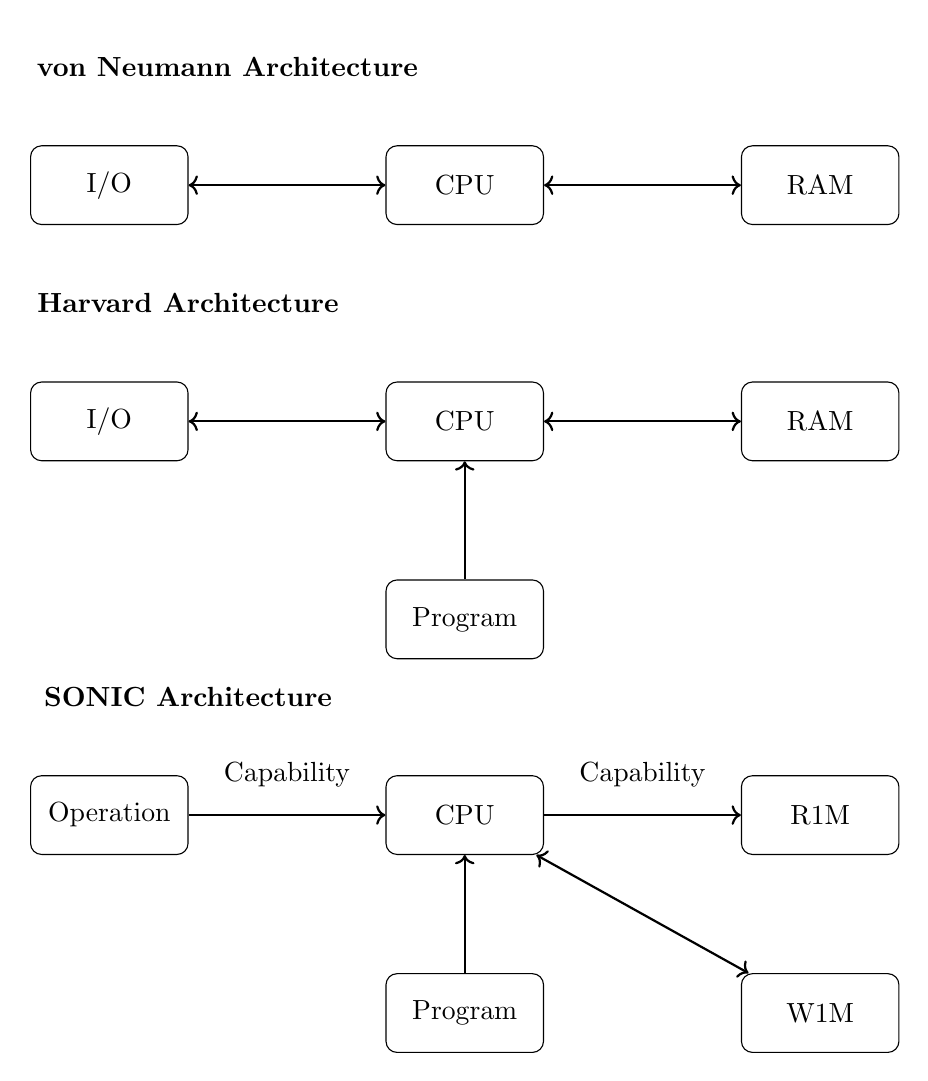
\begin{tikzpicture}[
        node distance=1.5cm and 2.5cm,
        every node/.style={draw, rounded corners, minimum width=2cm, minimum height=1cm, align=center},
        capability/.style={->, thick},
        dataflow/.style={<->, thick},
        flow/.style={->, thick}
    ]
    
    % von Neumann Architecture
    \node[draw=none, align=left] at (-4.5,3.5) {\textbf{von Neumann Architecture}};
    \node (IO1) at (-6,2) {I/O};
    \node (CPU1) [right=of IO1] {CPU};
    \node (RAM1) [right=of CPU1] {RAM};
    
    \draw[dataflow] (IO1) -- (CPU1);
    \draw[dataflow] (CPU1) -- (RAM1);
    
    % Harvard Architecture
    \node[draw=none, align=left] at (-5,0.5) {\textbf{Harvard Architecture}};
    \node (IO2) at (-6,-1) {I/O};
    \node (CPU2) [right=of IO2] {CPU};
    \node (RAM2) [right=of CPU2] {RAM};
    \node (Program1) [below=of CPU2] {Program};
    
    \draw[dataflow] (IO2) -- (CPU2);
    \draw[dataflow] (CPU2) -- (RAM2);
    \draw[flow] (Program1) -- (CPU2);
    
    % SONIC Architecture
    \node[draw=none, align=left] at (-5,-4.5) {\textbf{SONIC Architecture}};
    \node (Operation) at (-6, -6) {Operation};
    \node (CPU3) [right=of Operation] {CPU};
    \node (R1M) [right=of CPU3] {R1M};
    \node (W1M) [below=of R1M] {W1M};
    \node (Program2) [below=of CPU3] {Program};
    
    \draw[capability] (CPU3) -- (R1M) node[midway, above, draw=none] {Capability};
    \draw[capability] (Operation) -- (CPU3) node[midway, above, draw=none] {Capability};
    \draw[dataflow] (CPU3) -- (W1M);
    \draw[flow] (Program2) -- (CPU3);
    
    \end{tikzpicture}

    \caption{Comparison of different computer architectures}
    \label{fig:arch}
\end{figure}
\begin{multicols}{2}


\subsection{Memory}\label{Memory}

The SONIC architecture supports two types of addressed memory:
\begin{description}
    \item[Read-once memory] (R1M), or \gls{destructible memory} $\mathcal{D}$, having capability-based access
    and used for storing \emph{owned state} accessible only by a valid actor providing a 256-bit
    \gls{authentication token};

    \item[Write-once memory] (W1M), or \gls{immutable memory} $\mathcal{I}$, which can be accessed by any
    party and is used to define a global contract state.
\end{description}

Both types of memory are made of addressable memory cells.
An address consists of a 256-bit id of operation and 16-bit output number
which creates the memory cell:

\begin{gather}
\mathbb{A} \triangleq \mathbb{N}^{32}_8 \times \mathbb{N}_{16} \\
\mathsf{a} \triangleq \langle \mathsf{Id}(c_i), j \rangle \in \mathbb{A}
\end{gather}

Memory data are based on \glspl{composed value} data type,
which is an ordered sequence of zero to four finite field elements:

\begin{equation}
\mathbb{V} \triangleq \bigcup_{n=0}^{4} \mathbb{F}_q^n
\end{equation}

\Gls{read-once memory} cells consist of a single \gls{composed value} $\sigma$,
an \gls{authentication token} $\alpha$, and an optional \gls{locking condition} $\mathcal{L}$:

\begin{gather}
\mathbb{D} \triangleq \mathbb{V} \times \mathbb{F}_q \times \{ \varnothing, \langle \mathbb{V}, \{ \varnothing, \mathbb{E} \} \rangle \} \\
\forall \mathsf{d}_i \in \mathcal{D}(\mathsf{a}) : \mathsf{d}_i \triangleq \langle \sigma, \alpha, \mathcal{L} \rangle \in \mathbb{D}
\end{gather}

A locking condition, when present as $\langle \xi, \ell \rangle \in \mathcal{L} \setminus \{ \varnothing \}$,
consists of an auxiliary data $\xi$ and an optional verification script entry point $\ell$.

The auxiliary data may be used by the codex verifier script or the custom locking script $\ell$
to check the satisfaction of the lock conditions with an input-specific witness,
which will come from the spending input.
For example, this may be the value of a public key, and the witness will have a signature,
while the script will validate the signature for that key.

The locking script, when present as $\varepsilon \in \ell \setminus \{ \varnothing \}$,
is an entry point into the AluVM program (see next section),
which should succeed on execution in order for the cell to be read and destroyed.

The destructible memory cell is destroyed on the first read operation
and cannot be accessed or referenced anymore.

\Gls{immutable memory} cells consist of a single \gls{composed value} $\varsigma$,
and an optional binary raw data $\mathcal{R}$, up to $2^{16}$ bytes:

\begin{gather}
\mathbb{I} \triangleq \mathbb{V} \times \{ \varnothing, \mathbb{N}_8^{[0; 2^{16})} \}_\preceq \\
\forall \mathsf{e}_i \in \mathcal{I}(\mathsf{a}) : \mathsf{e}_i \triangleq \langle \varsigma, \mathcal{R} \rangle \in \mathbb{I}
\end{gather}

The raw data do not participate in the validation process and thus are never arithmetized.
Their purpose is to provide more context information for the user, and they are parsed and processed
using ABI rules and the standard library code (see the RGB-1010 standard \cite{RGB1010}).


\subsection{Program}\label{Program}

AluVM operates as a Turing machine, running on a ``tape'' of a SONIC program,
with the following modifications:

\begin{itemize}
\item the machine can't change the cells on the tape (the program is read-only);
\item it has access to external data outside of the tape:
    \begin{itemize}
    \item current contract operation,
    \item addressable (see Section \ref{Memory});
    \end{itemize}
\item its execution is bounded by so-called \emph{complexity measure};
  each execution of an instruction increase complexity counting register in AluVM virtual CPU,
  and when the value exceeds a limit provided as a part of a contract Codex (see Section \ref{Codex}),
  it halts, ending in a failed state.
\end{itemize}

The machine executes a single instruction at each step.
The complete list of all instructions and their encodings,
as well as information about registers (i.e., Instruction Set Architecture),
is given in Annex \ref{AnnexA}.

AluVM comes with a set of special-purpose control registers.
Three of these registers influence the halting conditions of the machine:

\begin{description}
\item[CH] Halting register. When set to \texttt{true}, halts the program when \textbf{CK} is set to the failed state.
\item[CK] Check register, which is set for any failure (accessing register in \texttt{None} state,
        zero division, etc.). Can be reset if \textbf{CH} is \texttt{false}.
\item[CO] Test register, which acts as a Boolean test result (also a carry flag).
        Its value is checked by branching and some halting instructions.
\item[CA] Complexity accumulator / counter.
        Each instruction has a computational complexity measure.
        This register sums up the complexity of the instructions executed.
\item[CL] Complexity limit. If this register has a value set, once \textbf{CA} reaches or exceeds its value,
        the VM will set \textbf{CK} to a failed state.
\end{description}

The program halts on the following conditions:

\begin{enumerate}
\item On an unconditional halting instruction execution (see table of all instructions);
\item On a conditional halting instruction execution
   \emph{if} the value of instruction-specific register (\textbf{CO} or \textbf{CK}) is set;
\item On any invalid operation (division by zero, accessing non-existing value or memory cell, etc.)
   \emph{if} the \textbf{CH} is set;
\item On a jump to an unknown location
   (unknown library id or an offset outside the bounds of the library code segment);
\item Once the complexity limit given in \textbf{CL} is exceeded,
   \emph{if} the \textbf{CL} register contains a value, and \textbf{CH} is set.
\end{enumerate}

The complexity limit \textbf{CL} and halting flag \textbf{CH} are initialized using contract parameters
from a Codex (see Section \ref{Codex}). When a complexity limit and halting are defined, an AluVM program
is guaranteed to halt; allowing termination analysis.

Execution of a program results in an execution trace consisting of instructions,
input values (values in registers before instruction was executed),
output values (new values in registers once the instruction is executed)
and hidden parameters, coming from the external data if they were accessed.
The execution trace may be encoded using elements of the finite field $\mathbb{F}_q$
and fed to a zk-STARK prover. Specific details of the encoding and selection of the zk-STARK prover
are beyond the scope of this document and are a subject of future work.

To run a program, AluVM must be provided with an unordered set of known \emph{libraries},
used by the program, and an \emph{entry point} 
$\mathsf{h} \triangleq \langle \mathsf{Id_{lib}} \in \mathbb{N}^{32}_8, p \in \mathbb{N}_{16} \rangle$,
consisting of a library id $\mathsf{Id_{lib}}$ and an offset $p$ in the library code segment.
The number of known libraries is unbounded; therefore, the complexity limit mechanism
is the only way to bound the computation of a program.
For information about the AluVM library, its structure, constraints, etc. please refer to the
documentation \cite{AluVM}.

\section{Contracts}

The contract is an instance of the RGB protocol. RGB consensus operates on the contract level,
and doesn't include (as of version I.0) any cross-contract functionality\footnote{%
However, one may still achieve cross-contract interaction outside of the consensus layer,
for instance using atomic swaps.}.

Since RGB operates as a partially-replicated state machine,
each party has a partial view over contracts, named \emph{local contract}. 
A local contract is defined as
\noindent
\begin{equation}
\mathsf{C} \triangleq \langle \mathsf{\Theta}, \mathcal{O} \setminus \{ \mathsf{c}_0 \} \rangle
\end{equation}
\noindent
where $\Theta$ is a contract issue and
$\mathcal{O}$ is the locally known part of the contract operations
(excluding the genesis operation $\mathsf{c}_0$ already present in $\Theta$, see below).

The \emph{issue} defines the \emph{unique} and \emph{global} properties of the contract;
it must be known to all parties (i.e., present in each \emph{local contract} instance) and
it is represented by a tuple
\noindent
\begin{equation}
\mathsf{\Theta} \triangleq \langle v, \mathsf{m}, \mathsf{k}, \mathsf{c}_0 \rangle
\end{equation}
\noindent
which components are defined in Table \ref{tab:contract}.

The commitment to the \emph{issue} data represents a unique and global \emph{contract id}
$\mathsf{Id}(\mathsf{C})$, or $\mathsf{C_{Id}}$.

The contract metadata $\mathsf{m}$ define contract-specific parameters, which include
(in the order of their position in the tuple):

\begin{enumerate}
\item boolean indicating whether the contract is a test contract,
\item a specific consensus layer 1 used by the contract,
\item ISO 8601 timestamp of the moment the contract is issued,
\item a set of feature flags (must be zeros for RGB-I.0),
\item optional name of the contract, which must start with a capital letter or a \texttt{\_} symbol,
  and may contain up to 99 ASCII letters, numbers, or \texttt{\_} symbol,
\item an identity string of the contract issuer, made of ASCII printable characters.
\end{enumerate}

\end{multicols}
\begin{table}[h]
\centering
\caption{Specification of symbols used in the RGB contract}\label{tab:contract}
\begin{tabular}{ l l c l }
\toprule
Symbol & Type & Value range & Meaning \\
\midrule
$v$ & $\mathbb{N}_8$ & constant $0$ & RGB issue data structure version \\
$\mathsf{m}$   & $\langle \mathbb{B}, \mathbb{N}_8, \mathbb{N}_{64}, \mathbb{B}^{48}, \mathbb{S}_*^{[1, 100)?}, \mathbb{S}_\mathsf{printable}^{[1, 4096)} \rangle$ & n/a & Contract metadata \\
$\mathsf{k}$   & See Section \ref{Codex} & n/a & Codex \\
$\mathsf{c}_0$ & See Section \ref{Operation} & n/a & Genesis operation \\
\bottomrule
\end{tabular}
\end{table}
\begin{multicols}{2}


\subsection{Codex}\label{Codex}

The codex is a set of parameters and rules that define the contract business logic
but do not define any form of a state. The \emph{contract business logic} does not mean
the way state transitions are created; instead, it defines how an arbitrary
state transition, created with any possible rules, gets validated. If it passes the validation,
its business logic is valid; otherwise, the state transition is invalid and does not apply.
This paves the way to huge scalability as well as much more compact zk-STARK proofs;
since any zk-proof just proves a result of a computation,
not specifying the exact way of performing the computation itself.
The mistake of blockchain developers was to put the actual state transition function in
the blockchain, which does not scale. Client-side validation, implemented in RGB, fixes that.

Thus, an RGB codex defines a state transition \emph{validation} functions
which are differentiated by a state transition type:
a single contract may have multiple forms of state transition,
which can be seen as mutating methods of the contract.

Next, a codex defines the following contract parameters:

\begin{itemize}
\item Specific finite field size, which defines finite field $\mathbb{F}_q$ order $q$ and
  bit dimensions for finite field type variables, denoted hereinafter as $\|q\|_\mathsf{bits}$;
\item cryptographic hash function used in commitment schemes;
\item specific single-use seal protocol, which also defines the subset of specific blockchain networks,
  and commitment schemes;
\item specific blockchain.
\end{itemize}

More formally, codex is a tuple
\noindent
\begin{equation}
\mathsf{k} \triangleq \langle v, n, d, t, f, q, \mathsf{\Gamma}, \mathsf{\Lambda}, V \rangle
\end{equation}
\noindent
which components are defined in Table \ref{tab:codex}.

\end{multicols}
\begin{table}[h]
\centering
\caption{Specification of symbols used in the RGB codex}\label{tab:codex}
\begin{tabular}{ l l c p{8cm} }
\toprule
Symbol & Type & Value range & Meaning \\
\midrule
$v$ & $\mathbb{N}_8$ & constant $0$ & RGB codex data structure version \\
$n$ & $\mathbb{N}_8^{[0, 255]}$ & n/a & Contract name, parsed as Unicode UTF-8 string \\
$t$ & $\mathbb{N}_{64}$ & any & ISO 8601 timestamp of codex creation \\
$f$ & $\mathbb{B}^{32}$ & constant $0$ & Feature flags (must be zeros in RGB-I.0) \\
$q$ & $\mathbb{Z}_q$ & $[0, \mathbb{Z}_q)$ & Finite field order \\
$\mathsf{\Gamma}$ & $\langle \mathbb{B}, \mathbb{B}, \mathbb{N}_{64} \rangle$ & n/a &  zk-AluVM configuration for state transition verification \\
$\mathsf{\Lambda}$ & $\langle \mathbb{B}, \mathbb{B}, \mathbb{N}_{64} \rangle$ & n/a & zk-AluVM configuration for memory access lock verification \\
$V$ & $\mathbb{N}_{16} \rightarrow \langle \mathbb{N}_8^{32}, \mathbb{N}_{16} \rangle$ & any & Entry points for verification functions using AluVM libs \\
\bottomrule
\end{tabular}
\end{table}

\begin{multicols}{2}

Configurations for a zk-AluVM are 3-tuples, which values correspond to:
\begin{enumerate}
\item Boolean flag indicating whether a VM must halt on the first occurrence of a failure;
\item Boolean indicating whether a complexity limit is set;
\item 64-bit natural number representing the complexity limit (of the \#2 is set).
\end{enumerate}

For details on complexity limits, please refer to AluVM documentation \cite{AluVM}.

A codex may be used by multiple contracts in the same way as a class,
defined with an OOP programming language, may instantiate multiple objects.

It is important to note that multiple contracts may reuse the same codex.
In this way, there appears a natural differentiation between contract issuers and codex developers,
with the former being specializing in financial services, assets, etc;
and the second being specialists in computer science.


\subsection{Contract State}

A \emph{local contract state} is fully defined by a set of its operations, $\mathcal{O}$.

Since RGB consensus needs to operate as a polynomial computer with a computation trace that is
arithmetizable as a set of polynomial constraints, the state of a contract at the level of
consensus must always be represented by a mathematical construct
made of elements of the finite field $\mathbb{Z}_q$, provided in the contract codex.
This state is not human-readable and must be processed using specific ABIs and interfaces
to be read by humans; however, this part is outside the consensus definition, belonging
to the RGB standard library, defined in the RGB-1010 standard \cite{RGB1010}.

Contract memory is a tuple $\langle \mathcal{D}, \mathcal{I} \rangle$,
consisting of destructible $\mathcal{D}$ and immutable $\mathcal{I}$ memory cells,
as described in Section \ref{Memory}.

\begin{itemize}
\item The destructible memory cells represent a \gls{read-once memory} (R1M),
  which is defined by contract operations with destructible outputs
  and is removed once accessed by any of the contract operations referencing it as one of its inputs.

\item The immutable memory cells represent a \emph{write-once multiple-access} memory (W1M),
  which is defined by contract operations immutable outputs
  and accessed by contract operations immutable inputs.
\end{itemize}

The state of the memory is defined as a result of executing the
$\mathsf{evaluate}: \mathcal{O} \rightarrow \langle \mathcal{D}, \mathcal{I} \rangle$ procedure,
as described in Section \ref{Evaluate}.

\columnbreak
\subsection{Contract Operation}\label{Operation}

Contract operation is a tuple
\begin{equation}
o_i \triangleq \langle \mathsf{c}_i, S_i, u_i \rangle
\end{equation}
\noindent
consisting of:
\noindent
\begin{itemize}
\item client-side information of contract state change, represented by a tuple $\mathsf{c}_i$;
\item an unordered map of seal definitions performed by an operation,
  $S_i(x): y_x \in \mathcal{Y_i} \rightarrow s_x$, where $s_x$ is a seal definition;
\item a seal closing witness information,
  which values must belong to a set of either unit value, or a specific witness $w_i$:
  $u_i \in \{ \varnothing, w_i \}$.
\end{itemize}

\end{multicols}
\begin{table}[h]
\centering
\caption{Specification of symbols used in the RGB operation}\label{tab:op}
\begin{tabular}{ l l l }
\toprule
Symbol & Type & Meaning \\
\midrule
$v$ & $\mathbb{N}_8$ & RGB consensus version (must be set to $0$) \\
$\mathsf{C_Id}$ & $\mathbb{N}_8^{32}$ & Contract id \\
$\phi$ & $\mathbb{N}_{16}$ & Call id \\
$\lambda$ & $\mathbb{N}_{16}$ & Nonce \\
$\Upsilon$ & $\mathbb{V}$ & Operation-level witness data (unrelated to single-use seal witness!) \\
$\mathcal{A}$ & $\{\mathbb{A} \times \mathbb{V}\}_\preceq^{[0, 2^{16})}$ & Destructible memory refs (input) \\
$\mathcal{B}$ & $\{\mathbb{A}\}_\preceq^{[0, 2^{16})}$ & Immutable memory refs (input) \\
$\mathcal{Y}$ & $\{\mathbb{D}\}_\preceq^{[0, 2^{16})}$ & Destructible memory declaration (output) \\
$\mathcal{Z}$ & $\{\mathbb{I}\}_\preceq^{[0, 2^{16})}$ & Immutable memory declaration (output) \\
\bottomrule
\end{tabular}
\end{table}
\begin{multicols}{2}

A client-side part of the operation is represented by a tuple
\noindent
\begin{equation}
\mathsf{c}_i \triangleq \langle v, \mathsf{C_Id}, \phi, \lambda, \Upsilon, \mathcal{A}, \mathcal{B}, \mathcal{Y}, \mathcal{Z} \rangle
\end{equation}
\noindent
which meaning is given in the table \ref{tab:op}.

The contract \emph{genesis} is a special type of operation, which contains no input:
\noindent
\begin{equation}
\mathsf{c}_0 \triangleq \langle \pi, \mathsf{k_{Id}}, \phi, \lambda, \Upsilon, \varnothing, \varnothing, \mathcal{Y}, \mathcal{Z} \rangle
\end{equation}

Each operation is identified by an operation id, $\mathsf{Id}(c_i)$, which is computed by
hashing serialized data for the client-side part of the operation,
as described in Section \ref{Commitments}. For genesis, the value of $\mathsf{k_{Id}}$
is replaced by the value of $\mathsf{C_{Id}}$ before the id of the operation is calculated.

\subsection{Set of Operations}

Each contract is defined by a partially ordered set of contract operations
$\mathcal{O} \triangleq \{ o_i \}$.
An element of this set is a tuple, $o_i \triangleq \langle c_i, S_i, u_i \rangle$, consisting of:
\begin{itemize}
\item client-side information of contract state change, $c_i$;
\item an unordered map of seal definitions performed by an operation, 
  $S_i: d_j \in \mathcal{Y}_i \rightarrow s_j$, where $s_j$ is a seal definition;
\item a seal closing witness information, 
  which values must belong to a set of either unit value, or a specific witness $w_i$: 
  $u_i \in \{ \varnothing, w_i \}$.
\end{itemize}

The set $\mathcal{O}$ has an initial element, called \emph{genesis} $o_0$, for which $u_i = \varnothing$.
There might be other operations for which $u_i = \varnothing$;
these operations are named \emph{state extensions}.

All operations in $\mathcal{O}$ are partially ordered by the rule

\begin{equation}
\begin{split}
o_i \prec o_j \Longleftrightarrow (\exists \ y \in \mathcal{Y}_i: y_\mathsf{addr} \in \mathcal{A}_j) \\
\vee (\exists \ x \in \mathcal{X}_i: x_\mathsf{addr} \in \mathcal{B}_j)
\end{split}
\end{equation}

which means that if there exists at least one output of $c_i$ which is used by $c_j$, or a global
state defined in $c_i$ that is read by $c_j$, then $o_i$ precedes $c_j$.

If $\mathcal{O}$ is not a directed acyclic graph and the above rule cannot be fulfilled without
collisions, the set of operations must be recognized as invalid.


\subsection{Evaluate Procedure}\label{Evaluate}

The contract state is evaluated using the following $\mathsf{evaluate}$ procedure applied to the set of
contract operations:

\begin{equation}\label{eq:evaluate}
\begin{split}
\mathsf{evaluate} \triangleq \forall o_i \in O: \\
(\forall \ a \in \mathcal{A}_i \ \exists! \ d \in \mathcal{D}_i: \mathsf{addr}(d) = a) \\
\wedge \ (\forall \ b \in \mathcal{B}_i \ \exists! \ e \in \mathcal{I}_i: \mathsf{addr}(e) = b) \\
\wedge \ \mathsf{verify}(w_i, \mathcal{Y}_i) \\
\wedge \ \mathsf{exec}(\mathsf{k}, \wp, \mathcal{I}_i, \mathcal{D}_i, c_i) \\
\Rightarrow 
\begin{cases}
    \mathcal{D}_{i+1} \mapsto (\mathcal{D}_i \setminus \mathcal{A}_i) \cup \mathcal{Y}_i, \\[6pt]
    \mathcal{I}_{i+1} \mapsto \mathcal{I}_i \cup \mathcal{Z}_i \\
\end{cases} \\
\nRightarrow \perp
\end{split}
\end{equation}

The $\mathsf{addr}$ procedure returns a memory address for a given memory cell.

The procedure $\mathsf{verify}$ performs the verification of a set of single-use seals and a witness
according to the LNPBP-8 standard \cite{LNPBP8}.

The $\mathsf{exec}$ procedure executes a verification program
and programs verifying fulfillment of individual lock conditions for the spent inputs,
and is provided with codex data, a set of known AluVM libraries $\wp$,
access to the memory and client-side operation data.
It succeeds if and only if at the halting of the AluVM machine its register \textbf{CK} is not set.

The first part of the algorithm (\ref{eq:evaluate}) checks whether an operation is correct and, in case of success,
the contract state is evolved (middle expression), or the operation must not be applied to the contract state,
and further validation must terminate with a failure.

\section{Commitments}\label{Commitments}

Commitments are created using binary data serialization using strict encoding \cite{strict}, specifically:
\begin{enumerate}
\item Numbers are serialized in little-endian format,
   using a number of bytes required to cover the bit dimension of the used numeric type.
\item Sum types (enums, including primitive types and those with associated data)
   are prefixed with an 8-bit tag.
\item Fixed-size arrays are encoded as is, with no prefixing.
\item Variable-size collections (objects representable as mathematical sets,
   either ordered or unordered, including sequences, partially ordered sets, ordered sets, maps)
   are prefixed with the size of the collection (cardinal number) in little-endian format,
   using the number of bytes which fully covers the maximal allowed collection dimension;
   followed by elements of the collection, serialized one after the other.
\item Totally ordered sets must be serialized in the order of the elements
\item Partially ordered and unordered sets do not participate in the RGB consensus.
\item Maps are serialized with elements corresponding to the key and value, composed as a tuple.
   The keys of the ordered maps must represent a totally ordered set
   and define the order of serialization of key-value tuples.
\item Product types (tuples) are serialized according to the order of their elements, with no prefixes.
\end{enumerate}

Data are serialized into hashers, which usually use a prefix (tagged) to uniquely codify
the type of the produced commitment. Collections may also be merklized, in order to allow
compact profs of inclusion. The complete structure of data serialization to produce commitments,
including tagged prefixes and details of merklization, is given in the Annex \ref{AnnexB}.


\section{Additional Information}
\subsection{RGB on Bitcoin}

When RGB is used on top of Bitcoin, the following parameters apply:

\begin{enumerate}
\item A \emph{contract issue} must reference the specific bitcoin blockchain \& network as a value for its
field $\mathsf{m}_2$ (\emph{layer 1} in contract metadata) using Table \ref{tab:layer1}.
\item TxO-based single-use seals must be used, as they are defined in the LNPBP-10 standard \cite{LNPBP10}.
\end{enumerate}

\begin{coltable}
\captionof{table}{Values for different Layer 1 used as a part of RGB contract metadata}\label{tab:layer1}
\begin{tabular}{r l}
\toprule
$\mathsf{m}_2$ value & Layer 1 \\
\midrule
$0$ & No layer 1 is used \\
$16$ & Bitcoin blockchain \\
$17$ & Liquid sidechain \\
$32$ & Prime \\
\bottomrule
\end{tabular}
\end{coltable}


\subsection{Security Assumptions}

The security of RGB consensus relies on the following two assumptions:

\begin{itemize}
\item The selected cryptographic hash function is collision-resistant;
\item The used single-use seal protocol is secure.
\end{itemize}

\subsection{Reference Implementation}

The reference implementation is provided in the repositories, and the libraries are listed
in the consensus section of the RGB-3 standard \cite{RGB3}.

\section{Acknowledgments}
The whole work was inspired by the earlier ideas of Peter Todd on the client-side validation \cite{CSV}
and single-use seals \cite{SUS1, SUS2} protocols. Giacomo Zucco was the first, who had analyzed its possible
applications and implications for Bitcoin blockchain and Lightning Network \cite{Zucco}.
Adam Borko had suggested ideas and critics on the zk-STARK compatibility of the protocol.
Olga Ukolova had provided a lot of feedback and comments during the protocol design phase.


\bibliographystyle{plain}
\begin{thebibliography}{9}
\bibitem{Szabo} \textsc{Smart Contracts} \url{https://nakamotoinstitute.org/library/smart-contracts/}
\bibitem{CSV} \textsc{Progress on Scaling via Client-Side Validation} \url{https://milan2016.scalingbitcoin.org/files/presentations/D2%20-%20A%20-%20Peter%20Todd.pdf}
\bibitem{SUS1} \textsc{Preventing Consensus Fraud with Commitments and Single-Use-Seals} \url{https://petertodd.org/2016/commitments-and-single-use-seals}
\bibitem{SUS2} \textsc{Building Blocks of the State Machine Approach to Consensus} \url{https://petertodd.org/2016/state-machine-consensus-building-blocks}
\bibitem{Zucco} \textsc{Giacomo Zucco and RGB Tokens Built on Bitcoin} \url{https://bitcoinmagazine.com/culture/video-interview-giacomo-zucco-rgb-tokens-built-bitcoin}
\bibitem{RGB3} \textsc{RGB-3 Standard}, \url{https://github.com/RGB-WG/RFC/blob/master/RGB-0003.md}
\bibitem{RGB6} \textsc{RGB-6 Standard}, \url{https://github.com/RGB-WG/RFC/blob/master/RGB-0006.md}
\bibitem{RGB1010} \textsc{RGB-1010 Standard}, \url{https://github.com/RGB-WG/RFC/blob/master/RGB-1010.md}
\bibitem{LNPBP8} \textsc{LNPBP-8}, \url{https://github.com/LNP-BP/LNPBPs/blob/master/lnpbp-0008.md}
\bibitem{LNPBP10} \textsc{LNPBP-10}, \url{https://github.com/LNP-BP/LNPBPs/blob/master/lnpbp-0010.md}
\bibitem{setbuilder} \url{https://en.wikipedia.org/wiki/Set-builder_notation}
\bibitem{strict} Strict Encoding, \url{https://docs.rs/strict_types}
\bibitem{Cairo}: \url{https://cairo-lang.org}
\bibitem{AluVM}: \url{https://docs.rs/aluvm}
\end{thebibliography}

\end{multicols}

\newpage

\appendix
\section{RGB Instruction Set Architecture}\label{AnnexA}

\begin{table}[h]
\centering
\caption{AluVM Control Flow Instruction Set Architecture}\label{tab:aluvm}
\begin{tabular}{l p{1cm} l p{1cm} p{1cm} p{1.5cm} p{1cm} p{1.5cm} p{5cm}}
\toprule
Op. code & Instr. byte & Args & Src. & Dst. & \textbf{CK} change & \textbf{CY} change & \textbf{CS/CP} (call stack) & Description \\
\midrule
NOP	    &0	&-  	&-      		&-                              &-	        &	  &		&Not an operation \\ \midrule
NOCO	&1	&-  	&\textbf{CO}	&$\mathbf{CO}$	                &-	      	&	  &		&Inverts \textbf{CO} \\ \midrule
CHCO	&2	&-  	&\textbf{CO}	&-                              &-	      	&	  &	    &Terminate if $\mathbf{CO} \stackrel{?}{=} \mathsf{true}$ \\ \midrule
CHCK	&3	&-  	&\textbf{CK}	&-                              &-	      	&	  &	    &Terminate if \textbf{CK} is in failed state \\ \midrule
FAIL	&4	&-  	&-         		&-                              &\textsf{failed}		&	  &	    &Set \textbf{CK} to failed state, terminates if \textbf{CH} is set \\ \midrule
RSET	&5	&-  	&\textbf{CK}	&$\mathbf{CO}, \mathbf{CK}$	    &-	      	&	  &		&Resets \textbf{CK}, sets \textbf{CO} to a previous \textbf{CK} value \\ \midrule
JMP	    &6	&$p$	&-		        &-                              &may fail	&inc  &		&Jump to location (unconditionally) \\ \midrule
JINE	&7	&$p$	&\textbf{CO}	&-                              &may fail	&inc  &		&Jump to location if $\mathbf{CO} \stackrel{?}{=} \mathsf{true}$ \\ \midrule
JIFAIL	&8	&$p$	&\textbf{CK}	&-                              &may fail	&inc  &		&Jump to location if \textbf{CK} is in failed state \\ \midrule
SH      &9	&$r$	&-              &-                              &may fail	&inc  &		&Relative jump \\ \midrule
SHNE	&10	&$r$	&\textbf{CO}	&-                              &may fail	&inc  &		&Relative jump if $\mathbf{CO} \stackrel{?}{=} \mathsf{true}$ \\ \midrule
SHFAIL	&11	&$r$	&\textbf{CK}	&-                              &may fail	&inc  &		&Relative jump if \textbf{CK} is in failed state \\ \midrule
EXEC	&12	&$h$	&-		        &-                              &may fail	&inc  & 	&Jump outside library \\ \midrule
FN  	&13	&$p$	&-		        &-                              &may fail	&     &inc  &Call inside library \\ \midrule
CALL	&14	&$h$	&-		        &-                              &may fail	&     &inc	&Call outside library \\ \midrule
RET 	&15	&-  	&-		        &-                              &-	      	&     &dec  &Return or finish program \\ \midrule
STOP	&16	&-  	&-		        &-                              &-	      	&     &     &Unconditionally stop program \\
\bottomrule
\end{tabular}
\end{table}

\newpage

\begin{table}[h]
\centering
\caption{\textbf{GFA256} Instruction Set Architecture Extension for AluVM}\label{tab:gfa256}
\begin{tabular}{l p{1cm} p{1cm} l l p{1.5cm} p{8cm}}
\toprule
Op. code & Instr. byte & Ext. half-byte & Src. & Dst. & \textbf{CK} change & Description \\
\midrule
TEST	&	64	&	0	&	\textbf{E}	&	\textbf{CO}	&		&	Tests if register contains a value and set \textbf{CO} accordingly.	\\ \midrule
CLR	&	64	&	1	&		&	\textbf{E}	&		&	Clear destination register value.	\\ \midrule
PUTD	&	64	&	2	&	$f \in \mathbb{F}_q$	&	\textbf{E}	&		&	Put a value to the destination register	\\ \midrule
PUTZ	&	64	&	3	&		&	\textbf{E}	&		&	Put zero value to the destination register	\\ \midrule
PUTV	&	64	&	4	&	\textsf{const}	&	\textbf{E}	&		&	Put predefined constant value to the destination register. The pre-defined constants are $1$, $2^{64}$, $2^{128}$ and $q$ (the order of the finite field taken from \textbf{FQ})	\\ \midrule
FITS	&	64	&	5	&	\textbf{E}, \textsf{bits}	&	\textbf{CO}	&	may fail	&	Test whether a value in a source register fits in the provided number of bits. Sets \textbf{CO} register to the results of the test. The \textsf{bits} value is an natural number representing the maximal number of lowest bits which may be set. If the source register does not contains a value, sets both \textbf{CO} and  \textbf{CK} to failed state, otherwise leaves the value in  \textbf{CK} unchanged.	\\ \midrule
MOV	&	65	&	6	&	\textbf{E}	&	\textbf{E}, \textbf{CO}	&		&	Moves (copies) value from the source to the destination register, overwriting the previous value in the destination. If the source has no value, the destination value is also cleared. Operation leaves the value in the source register unaffected, and does not change the values in \textbf{CO} and \textbf{CK} registers.	\\ \midrule
EQ	&	66	&	7	&	\textbf{E}, \textbf{E}	&	\textbf{CO}	&	may fail	&	Sets \textbf{CO} to the result of register equivalence test. If both registers do not contain a value, sets \textbf{CK} to failed state.	\\ \midrule
NEG	&	67	&	-	&	\textbf{E}	&	\textbf{E}	&	may fail	&	Take the value from the source register, negate using finite-field modulo arithmetics, and put the result into the destination register. If the source register has no value \textbf{CK} is set to failed state.	\\ \midrule
ADD	&	68	&	-	&	\textbf{E}, \textbf{E}	&	\textbf{E}	&	may fail	&	Add values of two registers using finite-field arithmetics and put the result into the first of the register. Do not detect overflows. If either of the source register does not contain a value, sets \textbf{CK} fo failed state.	\\ \midrule
MUL	&	69	&	-	&	\textbf{E}, \textbf{E}	&	\textbf{E}	&	may fail	&	Multiply values of two registers using finite-field arithmetics and put the result into the first of the register. Do not detect overflows. If either of the source register does not contain a value, sets \textbf{CK} fo failed state.	\\
\bottomrule
\end{tabular}
\end{table}

The \textbf{GFA256} ISA defines \textbf{FQ} constant (read-only) register,
which contains the order $q$ of the used finite field $\mathbb{F}_q$; and 
16 general registers to store finite field element values,
from \textbf{E1} to \textbf{E8}, and from \textbf{EA} to \textbf{EH}.
All registers are equivalent in their functionality and are represented as \textbf{E} in the table above.

\newpage

\begin{table}[h]
\centering
\caption{\textbf{USONIC} Instruction Set Architecture Extension for AluVM}\label{tab:usonic}
\begin{tabular}{l p{1cm} l l p{7cm}}
\toprule
Op. code & Instr. byte & Src. & Dst. & Description \\
\midrule
CKNXIRO	&128	&$\mathcal{A}, \mathbf{UI1}$	&\textbf{CO}	&Sets \textbf{CO} to the result of check $\mathbf{UI1} < \| \mathcal{A} \|$ \\ \midrule
CKNXIAO	&129	&$\mathcal{B}, \mathbf{UI2}$	&\textbf{CO}	&Sets \textbf{CO} to the result of check $\mathbf{UI2} < \| \mathcal{B} \|$ \\ \midrule
CKNXORO	&130	&$\mathcal{Y}, \mathbf{UI3}$	&\textbf{CO}	&Sets \textbf{CO} to the result of check $\mathbf{UI3} < \| \mathcal{Y} \|$ \\ \midrule
CKNXOAO	&131	&$\mathcal{Z}, \mathbf{UI4}$	&\textbf{CO}	&Sets \textbf{CO} to the result of check $\mathbf{UI4} < \| \mathcal{Z} \|$ \\ \midrule
LDW	    &132	&$\Upsilon$	                    &              	&Load operation witness data (not the same as single-use seal witness!) to \textbf{EA-ED} registers. \\ \midrule
LDIW	&133	&$\mathsf{d}_\varpi: \mathsf{addr}(\mathsf{d}_\sigma) = a_\mathbf{UI1}$	&	&Load a destructible input-specific witness for the current input number (determined by the value in \textbf{UI1}) to \textbf{EA-ED} registers. 
The operation is idempotent and does not update the value of \textbf{UI1} register. It also sets \textbf{CO} to indicate whether the input matching \textbf{UI1} value is present. \\ \midrule
LDIL	&134	&$\mathsf{d}_\varpi: \mathsf{addr}(\mathsf{d}_\xi) = a_\mathbf{UI1}$	&	&Load a destructible input-specific auxiliary locking conditions for the current input number (determined by the value to the \textbf{UI1}) to \textbf{EA-ED} registers. 
The operation is idempotent and does not update the value of \textbf{UI1} register. It also sets \textbf{CO} to indicate whether the input matching \textbf{UI1} value is present. \\ \midrule
LDIT	&135	&$\alpha_\mathbf{UI1}$	        &\textbf{CO}	&Load a destructible input authorization token $\alpha$ for the current input number (determined by the value in \textbf{UI1}) to \textbf{EA}. The operation also sets \textbf{EB} to either $0$ (if a custom lock script is not present) or $1$, if it is present.
The operation is idempotent and does not update the value of \textbf{UI1} register. It also sets \textbf{CO} to indicate whether the input matching \textbf{UI1} value is present. \\ \midrule
LDIRO	&136	&$\mathsf{d}_\sigma: \mathsf{addr}(\mathsf{d}_\sigma) = \mathsf{a}_\mathbf{UI1}$	&\textbf{EA-ED, CO}	&Load the destructible memory cell referenced by the next operation input to \textbf{EA-ED} registers. Sets \textbf{CO} to indicate whether the next element was present. \\ \midrule
LDIAO	&137	&$\mathsf{e}_\varsigma: \mathsf{addr}(\mathsf{e}_\varsigma) = \mathsf{b}_\mathbf{UI1}$	&\textbf{EA-ED, CO}	&Load the immutable memory cell referenced by the next operation input to \textbf{EA-ED} registers. Sets \textbf{CO} to indicate whether the next element was present. \\ \midrule
LDORO	&138	&$\sigma(\mathsf{y}_\mathbf{UI2})$	&\textbf{EA-ED, CO}	&Load next destructible operation output value to \textbf{EA-ED} registers. Sets \textbf{CO} to indicate whether the next element was present. \\ \midrule
LDOAO	&139	&$\varsigma(\mathsf{z}_\mathbf{UI2})$	&\textbf{EA-ED, CO}	&Load next immutable operation output value to \textbf{EA-ED} registers. Sets \textbf{CO} to indicate whether the next element was present. \\ \midrule
RSTIRO	&140	&-	&\textbf{UI1}	&Resets iterator over the input descructible memory cells by setting \textbf{UI1} to zero. \\ \midrule
RSTIAO	&141	&-	&\textbf{UI2}	&Resets iterator over the input immutable memory cells by setting \textbf{UI2} to zero. \\ \midrule
RSTORO	&142	&-	&\textbf{UI3}	&Resets iterator over the output descructible memory cells by setting \textbf{UI3} to zero. \\ \midrule
RSTOAO	&143	&-	&\textbf{UI4}	&Resets iterator over the output immutable memory cells by setting \textbf{UI4} to zero. \\
\bottomrule
\end{tabular}
\end{table}

All \textbf{USONIC} instructions do not take arguments. None of them changes the value in \textbf{CK}.


\newpage
\section{Commitments Specification}\label{AnnexB}
% Appendix II content here

\newpage
\section{}\label{AnnexC}
\printglossaries

\end{document}
